\subsection{2D Lighting}
\label{sub:2D Lighting}
\subsubsection{研究背景}

市面上不管 3D 或 2D 遊戲都會有光以及 RayCasting 的效果,而引擎應該要提供類似的功能。
在一款2D遊戲裡我們希望能有的效果是,有燈光的地方以及玩家在的地方是有視野的,其他地方是黑的,又或者是其他地方比較暗,玩家及其他地方有光的地方比較亮。

\subsubsection{效果}

而光一般會有以下三種效果

\begin{itemize}
\item{光衰減}
\item{照亮世界}
\item{Ray-Casting}
\end{itemize}

\subsubsection{實作}

\subsubsection{光衰減}
我們是在GPU計算光的。光在光源的位置是最亮的,之後距離光源越遠光的強度會越來越弱。
因此我們會需要知道光源的位置,接著計算每個 pixel 與光源之間的距離,利用這個距離計算出光的衰減。

\begin{lstlisting}
#version 450 core
out vec4 FragColor;

in vec2 v_LightPosition;
in vec4 v_Color;
in float v_Constant;
in float v_Linear;
in float v_Quadratic;

void main()
{
    // 獲取每個pixel
    vec2 pixel = vec2(gl_FragCoord.x, gl_FragCoord.y);
    // 計算每個pixel到光源的距離
    float distance = length(v_LightPosition - pixel.xy);
    // 如過大於光半徑則丟棄
    if(distance > v_Radius) discard;
    // 根據強度以及距離計算強度
    float attenuation = 1 / (1 + distance * 1/v_Strength);
    // 將光衰減乘上光顏色
    vec4 color = vec4(attenuation, attenuation, attenuation, pow(attenuation, 3)) * v_Color;

    FragColor = color;
}
\end{lstlisting}

\begin{figure}[h]
    \begin{center}
    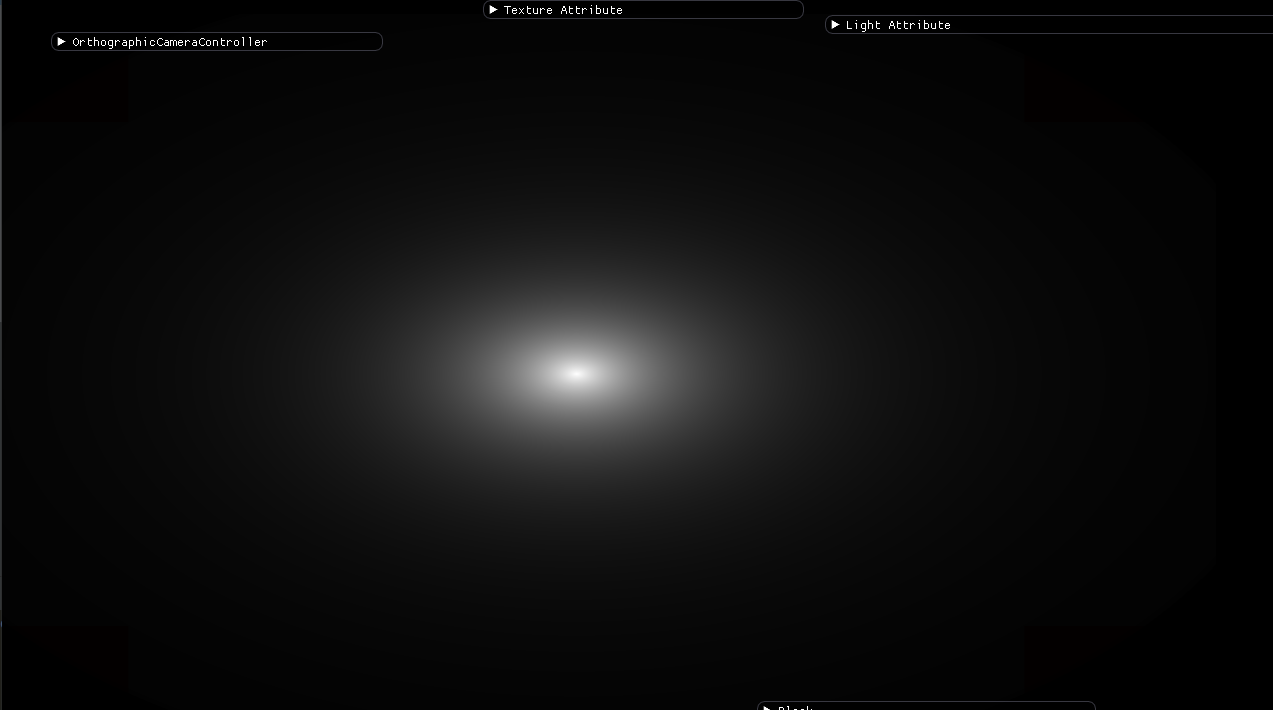
\includegraphics[width=0.6\textwidth]{./resources/2D-Lighting/attenuation.png}
    \end{center}
\caption{光衰減}
\label{fig:attenuation}
\end{figure}

獲取當前窗口所有座標,接著將傳入的lightPosition與每個pixel與光源計算距離,若距離大於所設定之影響半徑則丟棄,之後帶入光衰減函數去計算。

\begin{equation} F_{att} = \frac{1.0}{K + D * \frac{1.0}{S}} \end{equation}

此光衰減函數定義了三個項,分別是:

\begin{itemize}
\item{常數項K (Constant)}
    \SubItem{通常保持1.0,目的是保證分母永遠不會比1來的小,否則距離越遠強度反而會越強}
\item{距離D (Linear)}
    \SubItem{此距離為每個 pixel 與光源的距離}
\item{強度S (Quadratict)}
    \SubItem{影響光的強度}
\end{itemize}

計算好當前pixel的強度之後,將他乘上光的顏色,就能夠得到當前pixel的顏色了

\subsubsection{照亮世界}

在2D的世界裡,要將兩張半透明的Texture混在一起最簡單的作法是將兩張Texture相乘。
利用這個想法,我們需要將物體與光分別畫在不同的Framebuffer上,之後將這兩個Framebuffer合併,這樣就能得到光照在物體上並變亮的效果出來。

\begin{lstlisting}
{
    worldFBO->bind();
    Renderer::DrawStuff();
    worldFBO->unbind();
    lightFBO->bind();
    Renderer::DrawLight();
    lightFBO->unbind();
    combineFBO(lightFBO, worldFBO);
}
\end{lstlisting}

將物體與光分別畫在不同的Framebuffer裡,接著再將兩張Texture用Shader將它相乘。

\begin{lstlisting}
#version 430 core
in vec2 v_TexCoord;

out vec4 color;
uniform sampler2D u_Textures;
uniform sampler2D u_Textures2;

void main()
{
    vec4 worldColor = texture(u_Textures, v_TexCoord);
    vec4 lightColor = texture(u_Textures2, v_TexCoord);
    // 分別將兩張Texture乘起來
    color = worldColor * lightColor;
}
\end{lstlisting}

\begin{figure}[h]
    \begin{subfigure}[b]{0.5\linewidth}
        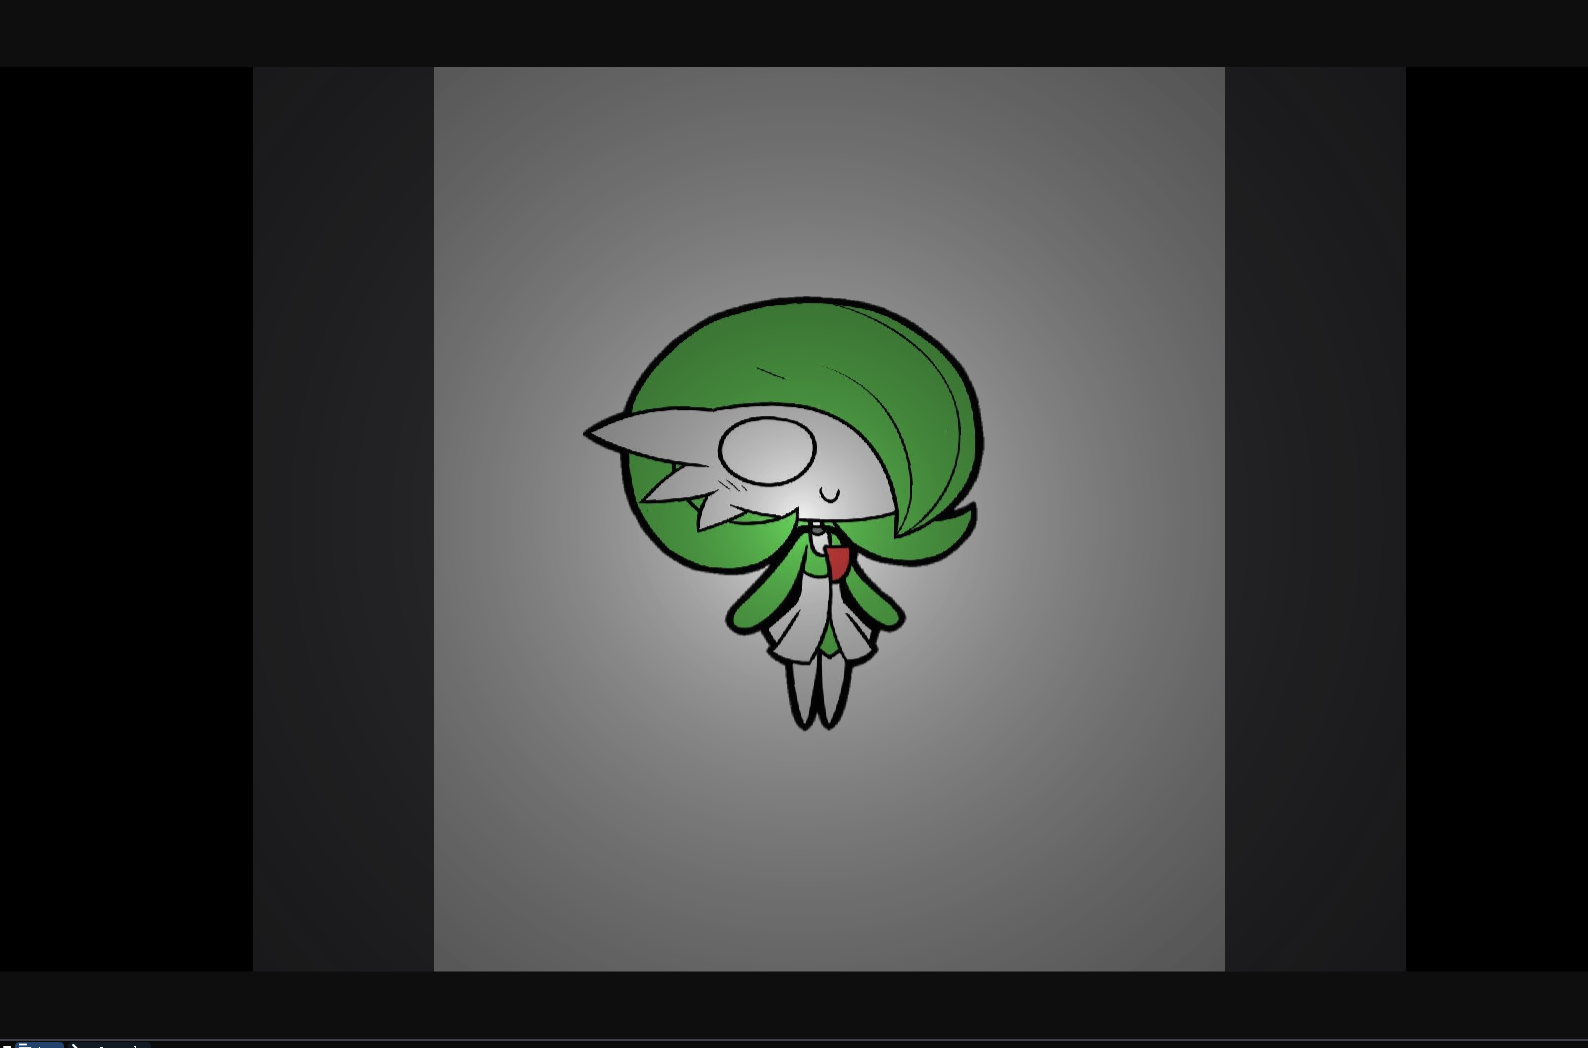
\includegraphics[width=\linewidth]{./resources/2D-Lighting/Light.png} 
        \caption{照亮世界}
    \end{subfigure}
    \begin{subfigure}[b]{0.5\linewidth}
        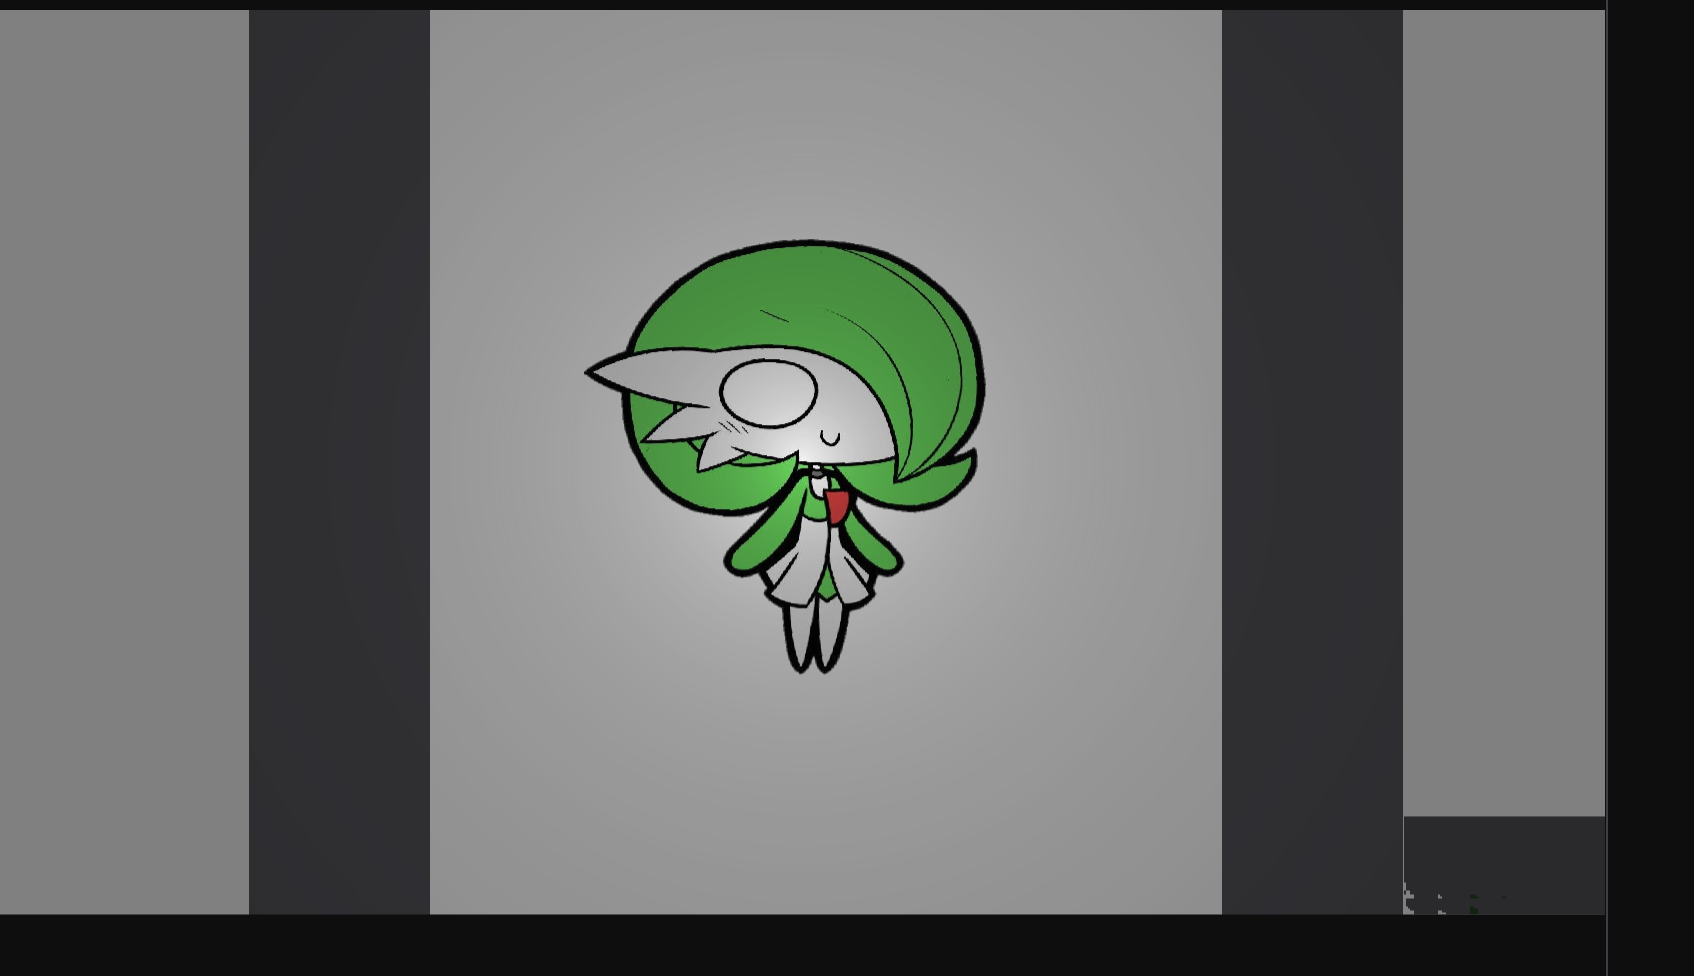
\includegraphics[width=\linewidth]{./resources/2D-Lighting/Ambient.png}
        \caption{Ambient}
    \end{subfigure}
\label{fig:Light}
\end{figure}

在光的那張Texture,光影響不到的地方的rgb是(0, 0, 0),而(0, 0, 0)不管乘上任何的顏色都會是(0, 0, 0),而有光的地方rgb不會是0,因此乘上世界的物體顏色就能將物體照亮物體,其餘地方將會是黑色

這樣只有有光的地方才能看到物體,沒有光的地方就是一片黑,若希望沒有光的地方不是全暗,仍能看到一些暗暗的背景的話,只需要在光的Framebuffer的背景上,畫上一張有顏色的矩形。如此一來,在光的framebuffer上我們會先有一個有顏色的背景,接著在這背景上畫上我們的光源,最後將這個與世界物體相乘,這樣沒有被光影響到的地方會乘上背景的顏色,就不會是全黑了。

\subsubsection{RayCasting}

光線照射到物體上,物體背後會產生陰影。

我們有光源位置以及兩個點(P1, P2),我們就能夠畫出陰影。點P1,P2所連成的直線背後是不可視的,因此要在後面畫上陰影(黑色)。我們取得P1以及P2的座標,利用向量計算光源到點p1的延伸點P3,以及光源到點P2的延伸點p4,用這四個點所圍成的四邊形即是陰影的部分。

運用這個道理,我們就能夠將世界物體的陰影給畫出來。在我們的引擎裡面,物體都是四邊形的。我們能夠輕易地找到座標畫出陰影。

若光源與P3 P4以及P2 P3畫陰影,會發生陰影蓋住物體的情況發生,因此需要找到距離光源較遠的邊。我們可以利用光到點的向量以及每條邊的法向量來幫助我們。

利用四個點我們能得到v1 v2 v3 v4四條向量,而我們分別找出這四條向量的法向量n1 n2 n3 n4,利用這四條法向量,與光源到點的向量座內積,如果大於零,方向基本相同,夾角在0°到90°之間則取兩點畫上陰影。

光與點P1所形成的向量與法向量n1做內積,小於0,則利用光源與點p1、p2做陰影。接著利用光與點p2所形成的向量語法向量n2做內積,以此類推。

\begin{figure}[h]
    \begin{subfigure}[b]{0.5\linewidth}
        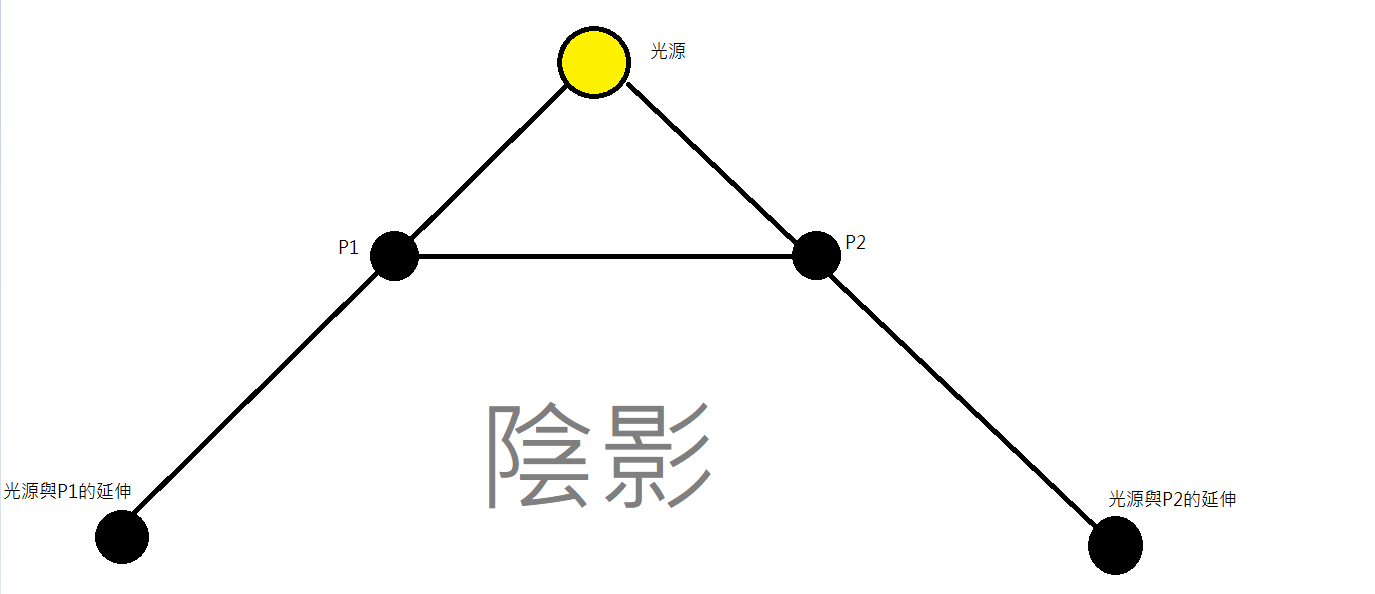
\includegraphics[width=\textwidth]{./resources/2D-Lighting/DrawShadow.png}
    \end{subfigure}
    \begin{subfigure}[b]{0.5\linewidth}
        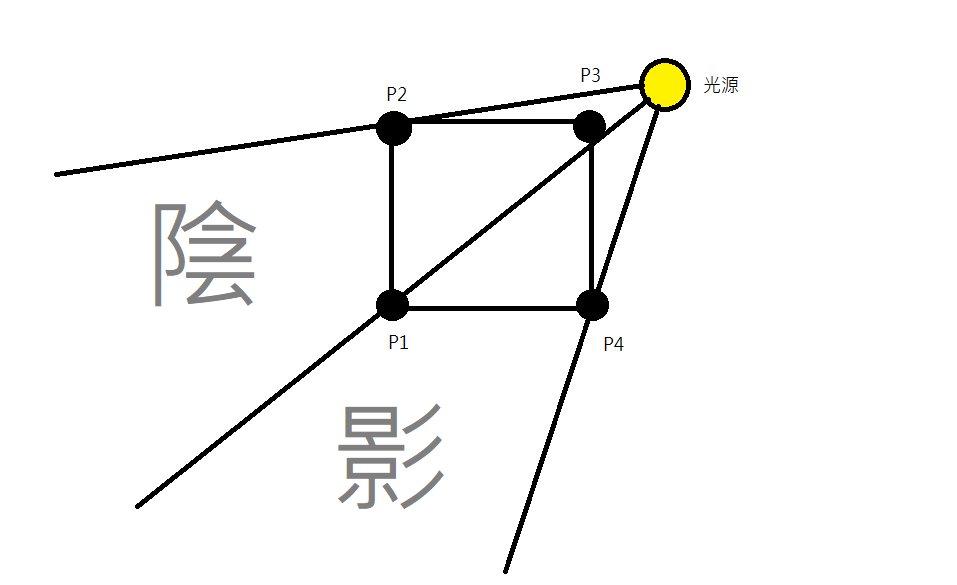
\includegraphics[width=\textwidth]{./resources/2D-Lighting/DrawShadow2.png}
    \end{subfigure}
\caption{對物體畫出陰影}
\label{fig:DrawShadow}
\end{figure}

\begin{lstlisting}
for(auto light : allLight)
{
    for(auto worldEntity : allWorldEntity)
    {
        // 獲取物體的點
        vector<glm::vec2> vertices = worldEntity->getVertices();
        
        for(int i = 0 ; i < vertices.size() ; i++)
        {
            // 目前的點
            glm::vec2 currentVertex  = vertices[i];
            // 下一個點,與目前的點連成一條線
            glm::vec2 nextVertex     = vertices[(i+1)%vertices.size()];
            // 計算兩點之向量
            glm::vec2 edge           = nextVertex - currentVertex;
            // 兩點向量之法向量
            glm::vec2 normal         = glm::vec2(-edge.y, edge.x);
            // 光源至目前點的向量
            glm::vec2 lightToCurrent = currentVertex - light->pos;
            
            // 計算內積判斷是否畫陰影
            if(glm::dot(normal, lightToCurrent) > 0)
            {
                Renderer::DrawShadow();
            }
        }
    }
    
    // Draw Light
}
\end{lstlisting}

\begin{figure}[h]
    \begin{subfigure}[b]{0.5\linewidth}
        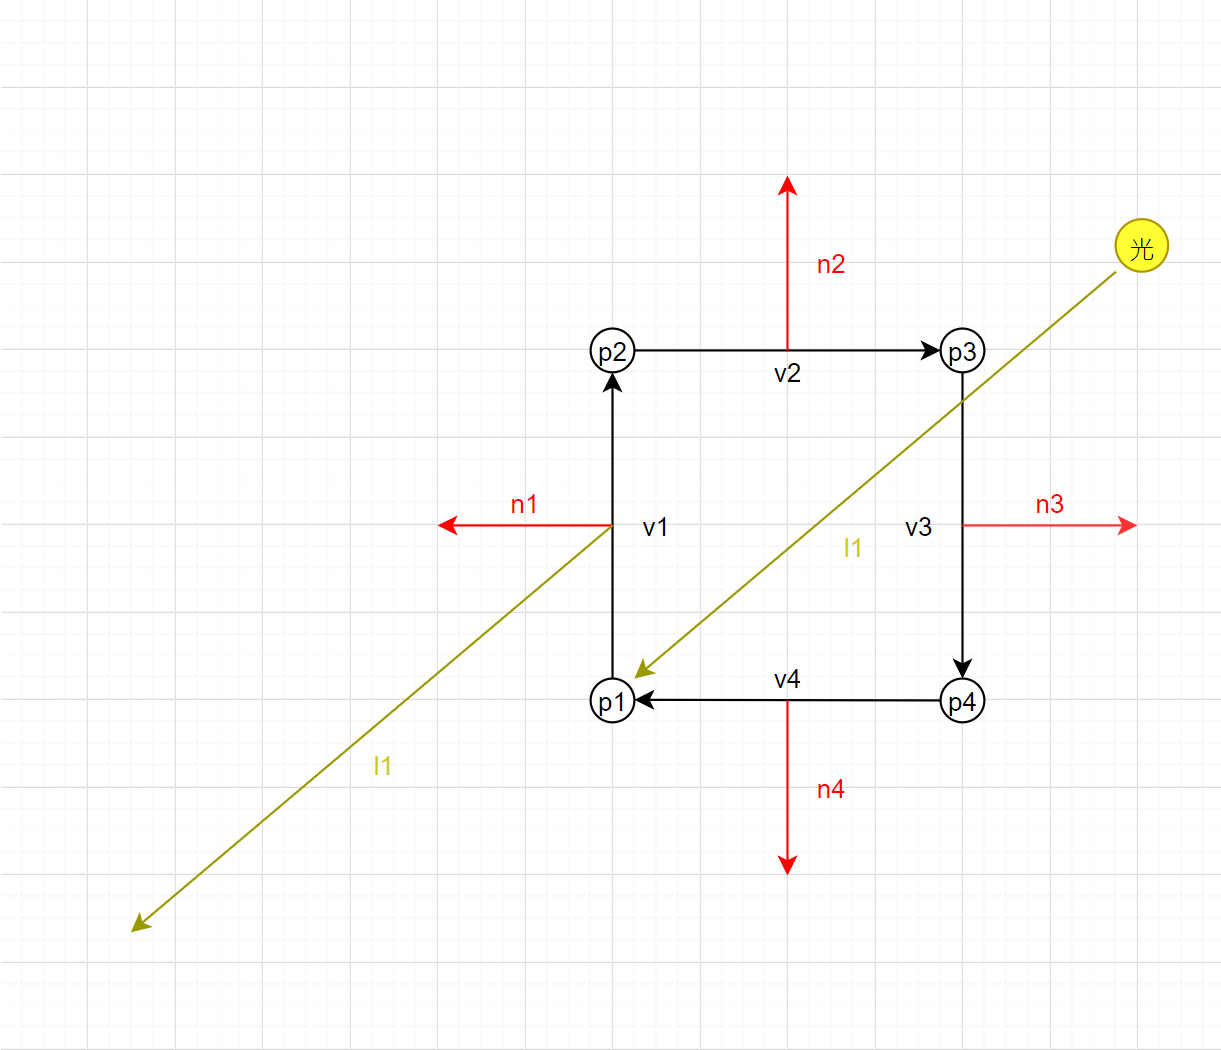
\includegraphics[width=\linewidth]{./resources/2D-Lighting/DrawShadow3.png} 
        \caption{判斷哪個邊要畫陰影}
    \end{subfigure}
    \begin{subfigure}[b]{0.5\linewidth}
        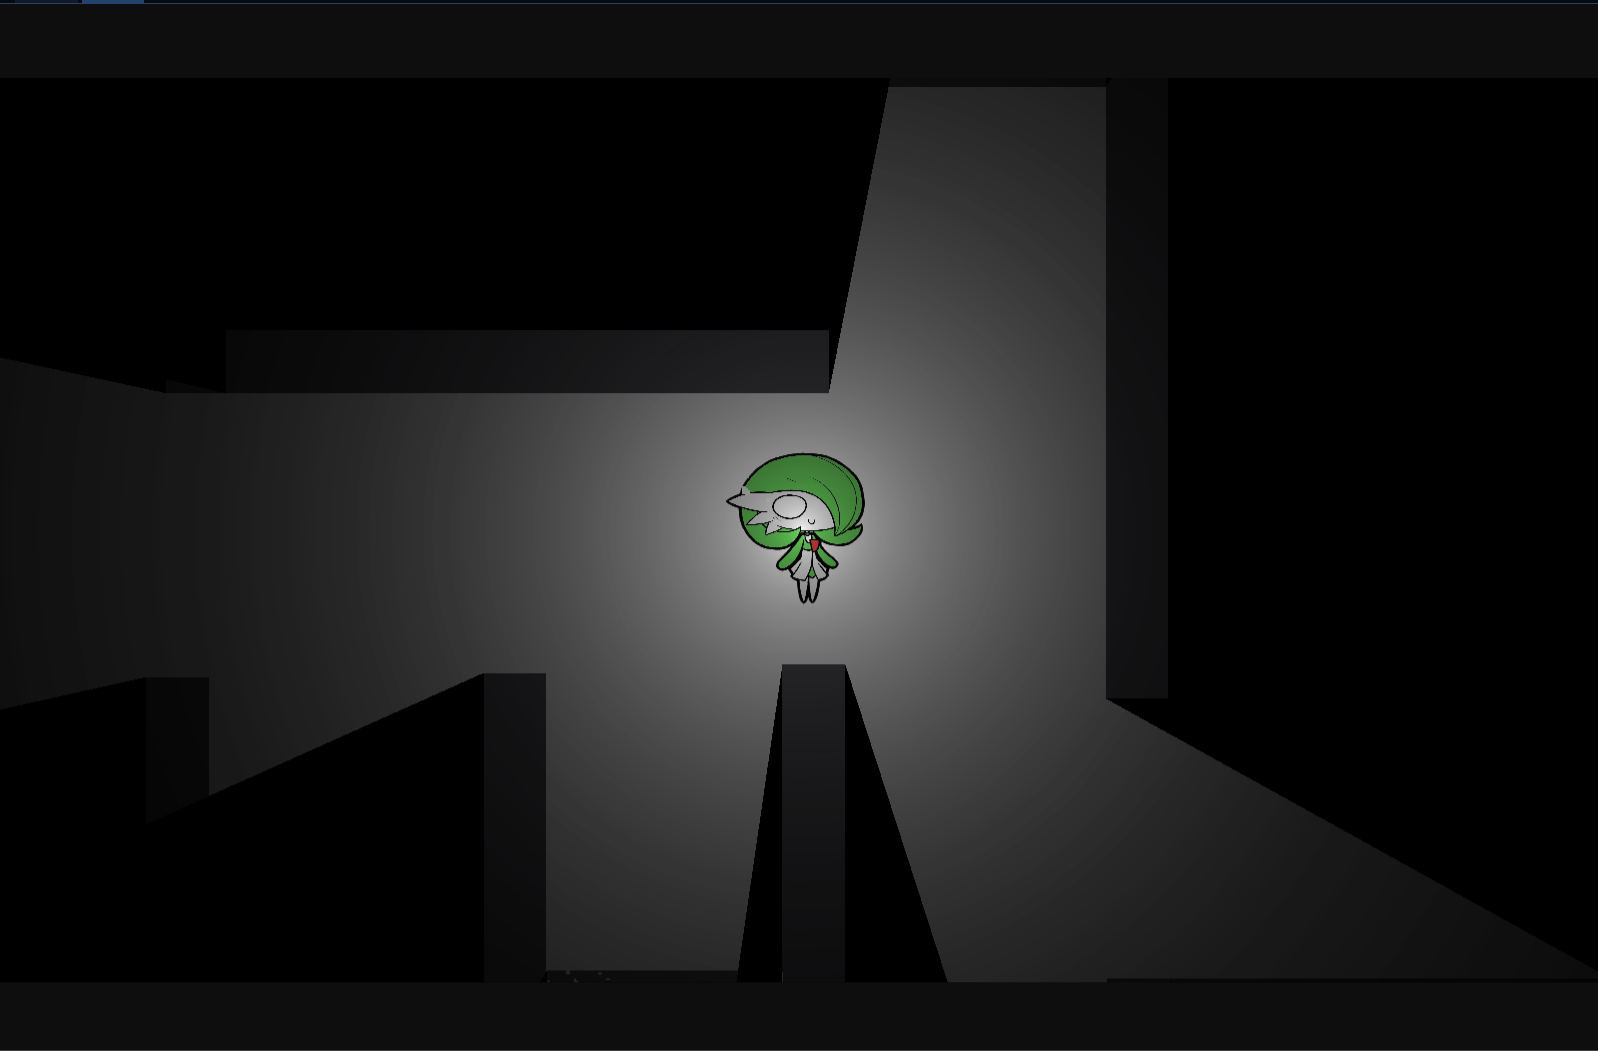
\includegraphics[width=\linewidth]{./resources/2D-Lighting/Ray-Cast.png} 
        \caption{Ray-Casting}
    \end{subfigure}
\label{fig:RayCasting}
\end{figure}

\subsubsection{結論}

擁有光之後,就能夠讓遊戲畫面更加的豐富,我們能夠調動世界的光暗,讓世界是暗的,只有擁有光源的地方能夠產生亮光。

\subsubsection{未來展望}

\begin{itemize}
\item{提供更多的光}
    \SubItem{目前只提供點光源}
\item{進入3D}
    \SubItem{將光照系統新增提供3D環境的光照}
\end{itemize}

\newpage
